% !TEX root = main.tex
\section{Architecture Framework}\label{sec:AAF}

%\subsection{Architecture Framework}\label{sec:archFram}

%\subsubsection{Overview}

An architecture framework is a
coordinated set of viewpoints, conventions, principles, and practices
for architecture description within a specific domain of application
or community of stakeholders~\cite{42010}.  More specifically, it is determined by: (i) a set of architecture-related concerns,
(i) a set of stakeholders holding those concerns, (ii) a set of architecture viewpoints which frame (i.e.,
cover) those concerns, and (iv) a set of model correspondence rules to impose constraints between
types of models and then demonstrate that constraints
are satisfied by the architecture. 
Then, an architecture framework establishes a common practice for creating, interpreting, analyzing and using architecture descriptions within a particular domain of application or stakeholder community, developing
architecture modelling tools and architecting methods, and establishing processes to facilitate communication, commitments and interoperation across multiple projects and/or organizations~\cite{42010}. 
Uses of architecture frameworks include, but are not limited to~\cite{42010}: 
%\eric{should we be specific about how this is useful for VCC? E.g. systematically creating and evolving architecture?}: 

\begin{itemize}
\item creating architecture descriptions; 
\item developing
architecture modelling tools and architecting methods; 
\item establishing processes to facilitate communication, commitments and interoperation across multiple projects and/or organizations.
\end{itemize}

An architecture framework is a prefabricated knowledge structure, identified by {\em architecture viewpoints}, that
architects use to organize an architecture description into {\em architecture views}.  The terms architecture view and architecture viewpoint are central to the standard~\cite{42010}:
{\em ``A viewpoint is a way of looking at systems; a view is the result of applying a viewpoint to a particular
system-of-interest''}. 
An {\em architecture viewpoint} encapsulates notations, conventions, methods, and techniques to
be used according to specific 
model kinds framing particular
concerns and for a particular audience of system stakeholders. 
The
concerns determine what the model kinds must be able to express: e.g.,
functionality, security, reliability, cost, deployment, etc.  
A model
kind determines the notations, conventions, methods and techniques to
be used. 
Viewpoints, defining the contents of each architecture view,
are built up from one or more model kinds and correspondence rules
linking them together to maintain consistency.
Viewpoints, like patterns and styles, are a form of reusable
architectural knowledge for solving certain kinds of architecture
description problems derived from best practices.  
Viewpoints
originated in the 1970s (in Ross' Structured Analysis) and refined in~\cite{Finkelstein+92}. Architecting methods often define one or
more viewpoints, e.g.~\cite{4+1,RozWooBook,ClementsBachmannEtAl03, Eeles-Cripps:2010}.


Many existing practices express architectures through collections of
models, and models are further organized into cohesive groups, called {\em views}. A view can be defined as a ``{\em work product expressing the architecture of a system from the perspective of specific system concerns}"~\cite{42010}.
As noted in the standard, the cohesion of a
group of models is determined by specific concerns, which are addressed by that group of models. Viewpoints refer to the conventions
for expressing an architecture with respect to a set of concerns.

For further discussion of the
content model and architecture frameworks mechanism,
see~\cite{Emery-Hilliard:2009}. 
Recent
frameworks include the ISO Reference Model for Open Distributed
Processing, GERAM (Generalized Enterprise Reference Architecture
and Methodology)~\cite{ISO15704}, DODAF (US Department of Defense Architecture
Framework)~\cite{DODAF}, TOGAF~\cite{TOGAF}, and MODAF~\cite{MODAF}. 
For an extensive survey of
frameworks, see~\cite{AFS}. 
    


%\subsection{Automotive domain}\label{sec:automotiveAFs}



%Automotive embedded systems are typically categorized into different domains, such as vehicle-centric functional domains
%(including powertrain control, chassis control, and active/passive safety systems) and
%passenger-centric functional domains (covering multimedia/telematics, body/comfort, and
%human machine interface (HMI))~\cite{Navet2008}. 
%Each functional domain needs to consider different stakeholders and
%system concerns~\cite{Yania}. %As an example, we can say that body domain supports the functioning of the airbag, wiper, and lighting
%%and other functions for the vehicle users, while the powertrain control enables the longitudinal propulsion
%%of the vehicle~\cite{Yania}). 
%However, at noted in~\cite{Yania} all the integrated functionalities must
%not jeopardize the key vehicle requirements of safety and efficiency.
%
%These considerations motivate the need of considering different viewpoints and views from the perspective of specific system concerns, which are relevant to one or more stakeholders. At the same time it is of key importance to identify and devise suitable connections among the various views and viewpoints.
%In other words, these considerations testify the need of an automotive architecture framework.

In this paper we use the template called \textit{Architecture Viewpoint Template} for specifying architecture viewpoints in
  accordance with ISO/IEC/IEEE~42010:2011, \textit{Systems and
    software engineering---Architecture description}\footnote{The template is called \textit{Architecture Viewpoint Template}, which is released under copyright \copyright\
2012--2014 by \href{http://www.iso-architecture.org/42010/templates/}%
{Rich Hilliard}. 
The template is licensed under a
Creative Commons Attribution 3.0 Unported License. The terms of use
are here: 
\url{http://creativecommons.org/licenses/by/3.0/}.}   


%%%% Version 2.1b %%%

%%%%%%%%%%
\section{\Fillin{Viewpoint Name}}\label{vp:template}
%%%%%%%%%%

\must{Provide the name for the viewpoint.}

If there are any synonyms or other common names by which this viewpoint is
known or used, record them here.


%%%%%%%%%%
\section{Overview} 
%%%%%%%%%%

Provide an abstract or brief overview of the viewpoint. 

Describe the viewpoint's key features.


%%%%%%%%%%
\section{Concerns and stakeholders} 
%%%%%%%%%%

Architects looking for an architecture viewpoint suitable for their
purposes often use the identified concerns and typical stakeholders to
guide them in their search.  Therefore it is important (and required
by the Standard) to document the concerns and stakeholders for which a
viewpoint is intended.

%%%%%%%%%%
\subsection{Concerns}\label{vp:concerns}
%%%%%%%%%%

\must{Provide a listing of architecture-relevant concerns to be framed by
this architecture viewpoint per \std{7a}.}

Describe each concern.

Concerns name ``areas of interest'' in a system.

\note{Following ISO/IEC/IEEE 42010, \textbf{system} is a shorthand for
  any number of things including man-made systems, software products
  and services, and software-intensive systems such as ``individual
  applications, systems in the traditional sense, subsystems, systems
  of systems, product lines, product families, whole enterprises, and
  other aggregations of interest''.}

Concerns may be very general (e.g., \textit{Reliability}) or quite
specific (\textit{e.g., How does the system handle network latency?}).
  
Concerns identified in this section are critical information for an
architect because they help her decide when this viewpoint will be
useful.

When used in an architecture description, the viewpoint becomes a
``contract'' between the architect and stakeholders that these
concerns will be addressed in the view resulting from this viewpoint.

It can be helpful to express concerns \emph{in the form of questions}
that views resulting from that viewpoint will be able to answer. E.g.,
\begin{itemize}
\item \textit{How does the system manage faults?}
\item \textit{What services does the system provide?}
\end{itemize}

\note{``In the form of a question'' is inspired by the television quiz
  show, \textit{Jeopardy!}}
 
\std{5.3} contains a candidate list of concerns that must be considered
when producing an architecture description. These can be considered
here for their relevance to the viewpoint being specified:
\begin{itemize}
\item What are the purpose(s) of the system-of-interest?
\item What is the suitability of the architecture for achieving the
  system-of-interest's purpose(s)?
\item How feasible is it to construct and deploy the
  system-of-interest?
\item What are the potential risks and impacts of the
  system-of-interest to its stakeholders throughout its life cycle?
\item How is the system-of-interest to be maintained and evolved?
\end{itemize}

See also: \std{4.2.3}.

%%%%%%%%%%
\subsection{Typical stakeholders} 
%%%%%%%%%%

\must{Provide a listing of the typical stakeholders of a system who
  are in the potential audience for views of this kind, per \std{7b}.}

Typical stakeholders would include those likely to read such views
and/or those who need to use the results of this view for another
task.

Stakeholders to consider include:
\begin{itemize}
\item users of a system; 
\item operators of a system; 
\item acquirers of a system;
\item owners of a system; 
\item suppliers of a system; 
\item developers of a system; 
\item builders of a system; 
\item maintainers of a system.
\end{itemize}

%%%%%%%%%%
\subsection{``Anti-concerns'' \Optional} 
%%%%%%%%%%

It may be helpful to architects and stakeholders to
document the kinds of issues for which this viewpoint is \emph{not
  appropriate or not particularly useful}.

Identifying the ``anti-concerns'' of a given notation or approach may
be a good antidote for certain overly used models and notations.

% \tbd{Examples!}



%%%%%%%%%%
\section{Model kinds+}\label{mk:list}
%%%%%%%%%%

\must{Identify each model kind used in the viewpoint per \std{7c}.}

In the Standard, each architecture view consists of multiple
architecture models. Each model is governed by a \textit{model kind}
which establishes the notations, conventions and rules for models of
that type.  See: \std{4.2.5, 5.5 and 5.6}.

Repeat the next section for each model kind listed here the viewpoint
being specified.


%%%%%%%%%%
\section{\Fillin{Model Kind Name}}\label{vp:mk}
%%%%%%%%%%

\must{Identify the model kind.}


%%%%%%%%%%
\subsection{\Fillin{Model Kind Name} conventions} 
%%%%%%%%%%

\must{Describe the conventions for models of this kind.}

Conventions include languages, notations, modeling techniques,
analytical methods and other operations. These are key modeling
resources that the model kind makes available to architects and
determine the vocabularies for constructing models of the kind and
therefore, how those models are interpreted and used.

It can be useful to separate these conventions into a \emph{language
  part}: in terms of a metamodel or specification of notation to be
used and a \emph{process part}: to describe modeling techniques used
to create the models and methods which can be used on the models that
result.  These include operations on models of the model kind.

The remainder of this section focuses on the language part. The next
section focuses on the process part.

The Standard does not prescribe \emph{how} modeling conventions are to
be documented.  The conventions could be defined:
\begin{description}
\item[I)] by reference to an existing notation or language (such as
  SADT, UML or an architecture description language such as ArchiMate
  or SysML) or to an existing technique (such as $M/M/4$ queues);
\item[II)] by presenting a metamodel defining its core constructs;
\item[III)] via a template for users to fill in;
\item[IV)] by some combination of these methods or in some other
  manner.
\end{description}

Further guidance on methods I) through III) is provided below.
 
Sometimes conventions are applicable across more than one model kind
-- it is not necessary to provide a separate set of conventions, a
metamodel, notations, or operations for each, when a single
specification is adequate.


%%%%%%%%%%
\subsubsection{I) Model kind languages or notations \Optional}
%%%%%%%%%%

Identify or define the notation used in models of the kind.

Identify an existing notation or model language or define one that can
be used for models of this model kind. Describe its syntax, semantics,
tool support, as needed.


%%%%%%%%%%
\subsubsection{II) Model kind metamodel \Optional} 
%%%%%%%%%%

A metamodel presents the AD elements that constitute the
vocabulary of a model kind, and their rules of combination. There are
different ways of representing metamodels (such as UML class diagrams, OWL,
eCore). The metamodel should present:
\begin{description}
\item[entities] What are the major sorts of conceptual elements that
  are present in models of this kind?
\item[attributes] What properties do entities possess in models of
  this kind?
\item[relationships] What relations are defined among entities in
  models of this kind?
\item[constraints] What constraints are there on entities, attributes
  and/or relationships and their combinations in models of this kind?
\end{description}

\note{Metamodel constraints should not be confused with architecture
  constraints that apply to the subject being modeled, not the
  notations used.}

In the terms of the Standard, entities, attributes, relationships are
\textit{AD elements} per \std{3.4, 4.2.5 and 5.7}.

In the \textit{Views-and-Beyond} approach~\cite{DSA:2010}, each
viewtype (which is similar to a viewpoint) is specified by a set of
elements, properties, and relations (which correspond to entities,
attributes and relationships here, respectively).

When a viewpoint specifies multiple model kinds it can be useful to
specify a single viewpoint metamodel unifying the definition of the
model kinds and the expression of correspondence rules.  When defining
an architecture framework, it may be helpful to use a single metamodel
to express multiple, related viewpoints and model kinds.

% \tbd{EXAMPLE -- In \cite{Hilliard:1999} and earlier work, we said that
%   all views are built from primitives called components, connections
%   and constraints which basically gives views a graph structure with
%   components as nodes and two types of edges (connections and
%   constraints). There are two issues with this: (\textit{1})
%   components and \textit{connectors} have taken on a specialized
%   meaning from the work by CMU and others \cite{Shaw-Garlan:1996};
%   (\textit{2}) this ur-ontology may be over-commiting for some views.}


%%%%%%%%%%
\subsubsection{III) Model kind templates \Optional}
%%%%%%%%%%

Provide a template or form specifying the format and/or content of
models of this model kind.

%% \tbd{EXAMPLE} 


%%%%%%%%%%
\subsection{\Fillin{Model Kind Name} operations \Optional} 
%%%%%%%%%%

Specify operations defined on models of this kind.

See~\S\ref{Opns} for further guidance.


%%%%%%%%%%
\subsection{\Fillin{Model Kind Name} correspondence rules}
%%%%%%%%%%

\must{Document any correspondence rules associated with the model
  kind.}

See~\S\ref{CRs} for further guidance.


%%%%%%%%%%
\section{Operations on views}\label{Opns}
%%%%%%%%%%

Operations define the methods to be applied to views and their models.
Types of operations include:

\begin{description}

\item[construction methods] are the means by which views are
  constructed under this viewpoint. These operations could be in the
  form of process guidance (how to start, what to do next); or work
  product guidance (templates for views of this type). Construction
  techniques may also be heuristic: identifying styles, patterns, or
  other idioms to apply in the synthesis of the view.

\item[interpretation methods] which guide readers to understanding
  and interpreting architecture views and their models.

\item[analysis methods] are used to check, reason about, transform,
  predict, and evaluate architectural results from this view,
  including operations which refer to model correspondence rules.

\item[implementation methods] are the means by which to design and
  build systems using this view.

\end{description}

Another approach to categorizing operations is from Finkelstein et
al. \cite{Finkelstein+1992}. The \emph{work plan} for a viewpoint
defines 4 kinds of actions (on the view representations):
\textit{assembly actions} which contains the actions available to the
developer to build a specification; \textit{check actions} which
contains the actions available to the developer to check the
consistency of the specification; \textit{viewpoint actions} which
create new viewpoints as development proceeds; \textit{guide actions}
which provide the developer with guidance on what to do and when.


%%%%%%%%%%
\section{Correspondence rules}\label{CRs}
%%%%%%%%%%

\must{Document any correspondence rules defined by this viewpoint or
  its model kinds.}

Usually, these rules will be across models or across views since,
constraints within a model kind will have been specified as part of
the conventions of that model kind.

See: \std{4.2.6 and 5.7}

%%\tbd{examples or specs}

%%%%%%%%%%
\section{Examples \Optional} 
%%%%%%%%%%

Provide helpful examples of use of the viewpoint for the reader
(architects and other stakeholders).


%%%%%%%%%%
\section{Notes \Optional} 
%%%%%%%%%%

Provide any additional information that users of the viewpoint may
need or find helpful.


%%%%%%%%%%
\section{Sources} 
%%%%%%%%%%

\must{Identify sources for this architecture viewpoint, if any,
  including author, history, bibliographic references, prior art, per
  \std{7e}.}



%According to the description above and to the standard~\cite{42010}, in this paper we will describe architecture viewpoints according to the following template:
%
In the following we report the template sections and an excerpt of the guidelines; please refer to the links above for a complete description of the template: 

\begin{itemize}
\item {\em Viewpoint Name}: name of the viewpoint. If there are any synonyms or other common names by which this viewpoint is
known or used, record them here.
\item {\em Overview}: Provide an abstract or brief overview of the viewpoint. 
Describe the viewpoint's key features.
\item {\em Concerns and stakeholders}: Architects looking for an architecture viewpoint suitable for their
purposes often use the identified concerns and typical stakeholders to
guide them in their search.  Therefore it is important (and required
by the Standard) to document the concerns and stakeholders for which a
viewpoint is intended.
%a listing of the architecture-related concerns framed by this viewpoint. This is
%crucial information for the Architect, because it helps her decide whether this
%viewpoint will be useful to apply to a given system of interest, and to
%communicate with its stakeholders.
\begin{itemize}
\item {\bf Concerns}: Describe each concern.
Concerns name ``areas of interest'' in a system.
Concerns may be very general (e.g., \textit{Reliability}) or quite
specific (\textit{e.g., How does the system handle network latency?}).
Concerns identified in this section are critical information for an
architect because they help her decide when this viewpoint will be
useful.
When used in an architecture description, the viewpoint becomes a
``contract'' between the architect and stakeholders that these
concerns will be addressed in the view resulting from this viewpoint.
It can be helpful to express concerns \emph{in the form of questions}
that views resulting from that viewpoint will be able to answer. E.g., {\em How does the system manage faults?} or {\em What services does the system provide?}
\item {\bf Typical stakeholders}: Provide a listing of the typical stakeholders of a system who
  are in the potential audience for views of this kind.
Typical stakeholders would include those likely to read such views
and/or those who need to use the results of this view for another
task.
\item {\bf Anti-concerns [Optional]} It may be helpful to architects and stakeholders to
document the kinds of issues for which this viewpoint is \emph{not
  appropriate or not particularly useful}.
Identifying the ``anti-concerns'' of a given notation or approach may
be a good antidote for certain overly used models and notations.
\end{itemize}
%\item {\em Anti-concerns [Optional]}: It can be useful to document the kinds of issues a viewpoint is not
%appropriate for. Articulating anti?concerns may be a good antidote for certain
%overly used notations.
%\item {\em Typical stakeholders}: The typical audience for views prepared using this viewpoint. This item should answer the question: Who
%are the usual stakeholders for this kind of view?
%\item {\bf Model Kind+} 
\item {\em Model Kind name\footnote{In the Standard, each architecture view consists of multiple
architecture models. Each model is governed by a \textit{model kind}
which establishes the notations, conventions and rules for models of
that type.  
Repeat the next section for each model kind listed here the viewpoint
being specified.}}:  Identify the model kind
%For each type of model used, describe the language or modeling techniques to
%be used. Each model language is a key modeling resource that the viewpoint
%makes available. Model languages provide the vocabularies for constructing the
%view. ISO/IEC 42010 does not specify how a modeling language is documented.
%It could be by reference to an existing modeling language (e.g., EAST-ADL or UML)
%or technique (e.g., M/M/4 queues); by providing a metamodel for the language
%to define the language's core constructs; via a template that users fill in; or by
%some combination of these methods.
\begin{itemize}
\item {\em Conventions}: Describe the conventions for models of this kind. Conventions include languages, notations, modeling techniques,
analytical methods and other operations. These are key modeling
resources that the model kind makes available to architects and
determine the vocabularies for constructing models of the kind and
therefore, how those models are interpreted and used.
The Standard does not prescribe \emph{how} modeling conventions are to
be documented.  The conventions could be defined:
\begin{description}
\item[I)] by reference to an existing notation or language (such as
  SADT, UML or an architecture description language such as ArchiMate
  or SysML) or to an existing technique (such as $M/M/4$ queues);
\item[II)] by presenting a metamodel defining its core constructs;
\item[III)] via a template for users to fill in;
\item[IV)] by some combination of these methods or in some other
  manner.
\end{description}
\item {\em Operations}: Specify operations defined on models of this kind.
\item {\em Correspondence rules}: Document any correspondence rules associated with the model
  kind.
\end{itemize}
\item {\em Operations on views}: Operations define the methods to be applied to views and their models.
Types of operations include:
\begin{description}
\item[construction methods] are the means by which views are
  constructed under this viewpoint. These operations could be in the
  form of process guidance (how to start, what to do next); or work
  product guidance (templates for views of this type). Construction
  techniques may also be heuristic: identifying styles, patterns, or
  other idioms to apply in the synthesis of the view.
\item[interpretation methods] which guide readers to understanding
  and interpreting architecture views and their models.
\item[analysis methods] are used to check, reason about, transform,
  predict, and evaluate architectural results from this view,
  including operations which refer to model correspondence rules.
\item[implementation methods] are the means by which to design and
  build systems using this view.
\end{description}
\item {\em Correspondence rules}: 
Document any correspondence rules defined by this viewpoint or
  its model kinds.
Usually, these rules will be across models or across views since,
constraints within a model kind will have been specified as part of
the conventions of that model kind.
%The viewpoint may specify model correspondence rules. Each one may be
%documented here.
%\item {\em Operations on views}: Operations define the methods which may be applied to views and their
%models. Operations can be divided into categories: Creation methods are the
%means by which views are prepared using the viewpoint. These could be in the
%form of process guidance (how to start, what to do next); or work product
%guidance (templates for views of this type); heuristics, styles, patterns, or other
%idioms. Interpretive methods provide the means by which views are to be
%understood by readers and system stakeholders. Analysis methods are used to
%check, reason about, transform, predict, apply and evaluate architectural
%results from this view. Implementation methods capture how to realize or
%construct systems using information from this view.
\item {\em Examples [Optional]}: 
Provide helpful examples of use of the viewpoint for the reader
(architects and other stakeholders).
\item {\em Notes [Optional]} Provide any additional information that users of the viewpoint may
need or find helpful.
%Optional. This section provides examples for the reader.
\item {\em Sources}: Identify sources for this architecture viewpoint, if any,
  including author, history, bibliographic references, prior art, etc.
%What are the sources for this viewpoint, if any? This may include author,
%history, literature references, prior art, etc.
\end{itemize}

%\eric{Should we relate this section to the status of the viewpoints we define here? E.g.:}
In this paper, we apply the viewpoint template above to describe three new viewpoints that we propose.
At the current state of our work, many details still need to be evaluated, thus we for example share model kind candidates as well as our experience on what kind of information these model kinds would need to provide, than presenting a clear definitions of models to be used.

\section{State of the art in Automotive Architecture Frameworks}\label{sec:automotiveAF}
Architecture frameworks have not been standardized in the automotive domain and automotive industry. 
However, some attempts exist and different types of architecture viewpoints and views have been introduced recently as part
of automotive architecture frameworks. 
A first attempt towards a standardized architectural foundation and automotive-specific
architecture framework is the Automotive
Architecture Framework (AAF) proposed in~\cite{Broy}. 
The purpose of AAF is to describe the entire vehicle system
across all functional and engineering domains and drive the thought process within the
automotive industry.
The AAF conforms to the ISO 42010 international standard~\cite{42010}, and therefore it is defined in terms of a set of viewpoints and views. 
%
%Figure~\ref{fig:aaf} shown the levels of architectures and architecture frameworks, spanning from the Meta Architecture Framework, which is the most generic layer that is fully independent of any type of system to develop, to the Product Architecture, which defines the architecture for a concrete product. 
%
  %
%\begin{figure}
%\begin{center}
%%  \vspace{-.3cm}
%  \includegraphics[width=.7\columnwidth]{figures/AAF.pdf}  
%  \caption{Automotive Architecture Framework (AAF) - Figure taken from~\cite{Broy}}
%%  \vspace{-.5cm}
%  \label{fig:aaf}
%    \end{center}
%\end{figure}
%
%Referring to~\cite{TUM-I0915}:
%
%The AAF is defined according to several levels; more details might be found at~\cite{TUM-I0915}. 
% of details as described below~\cite{TUM-I0915}:
%
%\begin{itemize}
%\item {\em Meta Architecture Framework} introduces terms like component, interface, view, viewpoint and concern. 
%\item {\em Common Architecture Framework} defines concepts, which are necessary for any kind of system. 
%%It is partitioned into three main parts, which are representing the total system at different layers of abstraction,
%%namely the Functional Architecture (functionality that the system offers
%% to its outside world - black-box and hardware agnostic), the Logical Architecture (decomposition of a system into a number of Logical Components - white-box and hardware agnostic) and the Technical Architecture (lower level of abstraction - runtime model, allocation, and hardware topology). 
%% % - see Figure~\ref{fig:abstractionDetails}.
%%\begin{itemize}
%%\item The Functional Architecture consists of a function hierarchy that contains the description of the functionality that the system offers
%% to its outside world. The description is black-box and is hardware agnostic. 
%%\item The Logical (Component) Architecture defines the decomposition of a system into a number of Logical Components, which interact
%%and cooperate to offer the functionality that is described in the Functional Architecture.
%%The description is then white-box, it can describe the functionality of a subsystem, and is hardware agnostic.
%%\item The Technical Architecture describes how the system that is specified by means of Logical Components can be integrated
%%into a given hardware platform. The system is presented from the  realization perspective. The technical architecture consists of three parts: The Runtime Model, the Allocation, and the Hardware Topology.
%%\end{itemize}
%\item {\em Domain-specific Architecture Framework for the Automotive Domain} defines the foundational framework providing a
%common denominator in terms of terminology, structure, methods, architecture models, guidance and rules. 
%%, ``{\em for
%%developing, representing, understanding, and comparing domain-specific product architectures across a
%%(virtual) development organization (i.e. Automotive value net)}"~\cite{TUM-I0915}.
%\item {\em Company X Architecture Framework} customizes the domain-specific Architecture
%Framework for a concrete company like Volvo cars, BMW or FIAT. We elaborate on the VCG architecture framework in Section~\ref{sec:VCGAF}.
%\item {\em Vehicle line architectures} defines the architecture for a specific product line.
%\item {\em Vehicle architectures} define the architecture for a specific product.
%\end{itemize}

 
%\begin{figure}
% \begin{center}
%%  \vspace{-.3cm}
%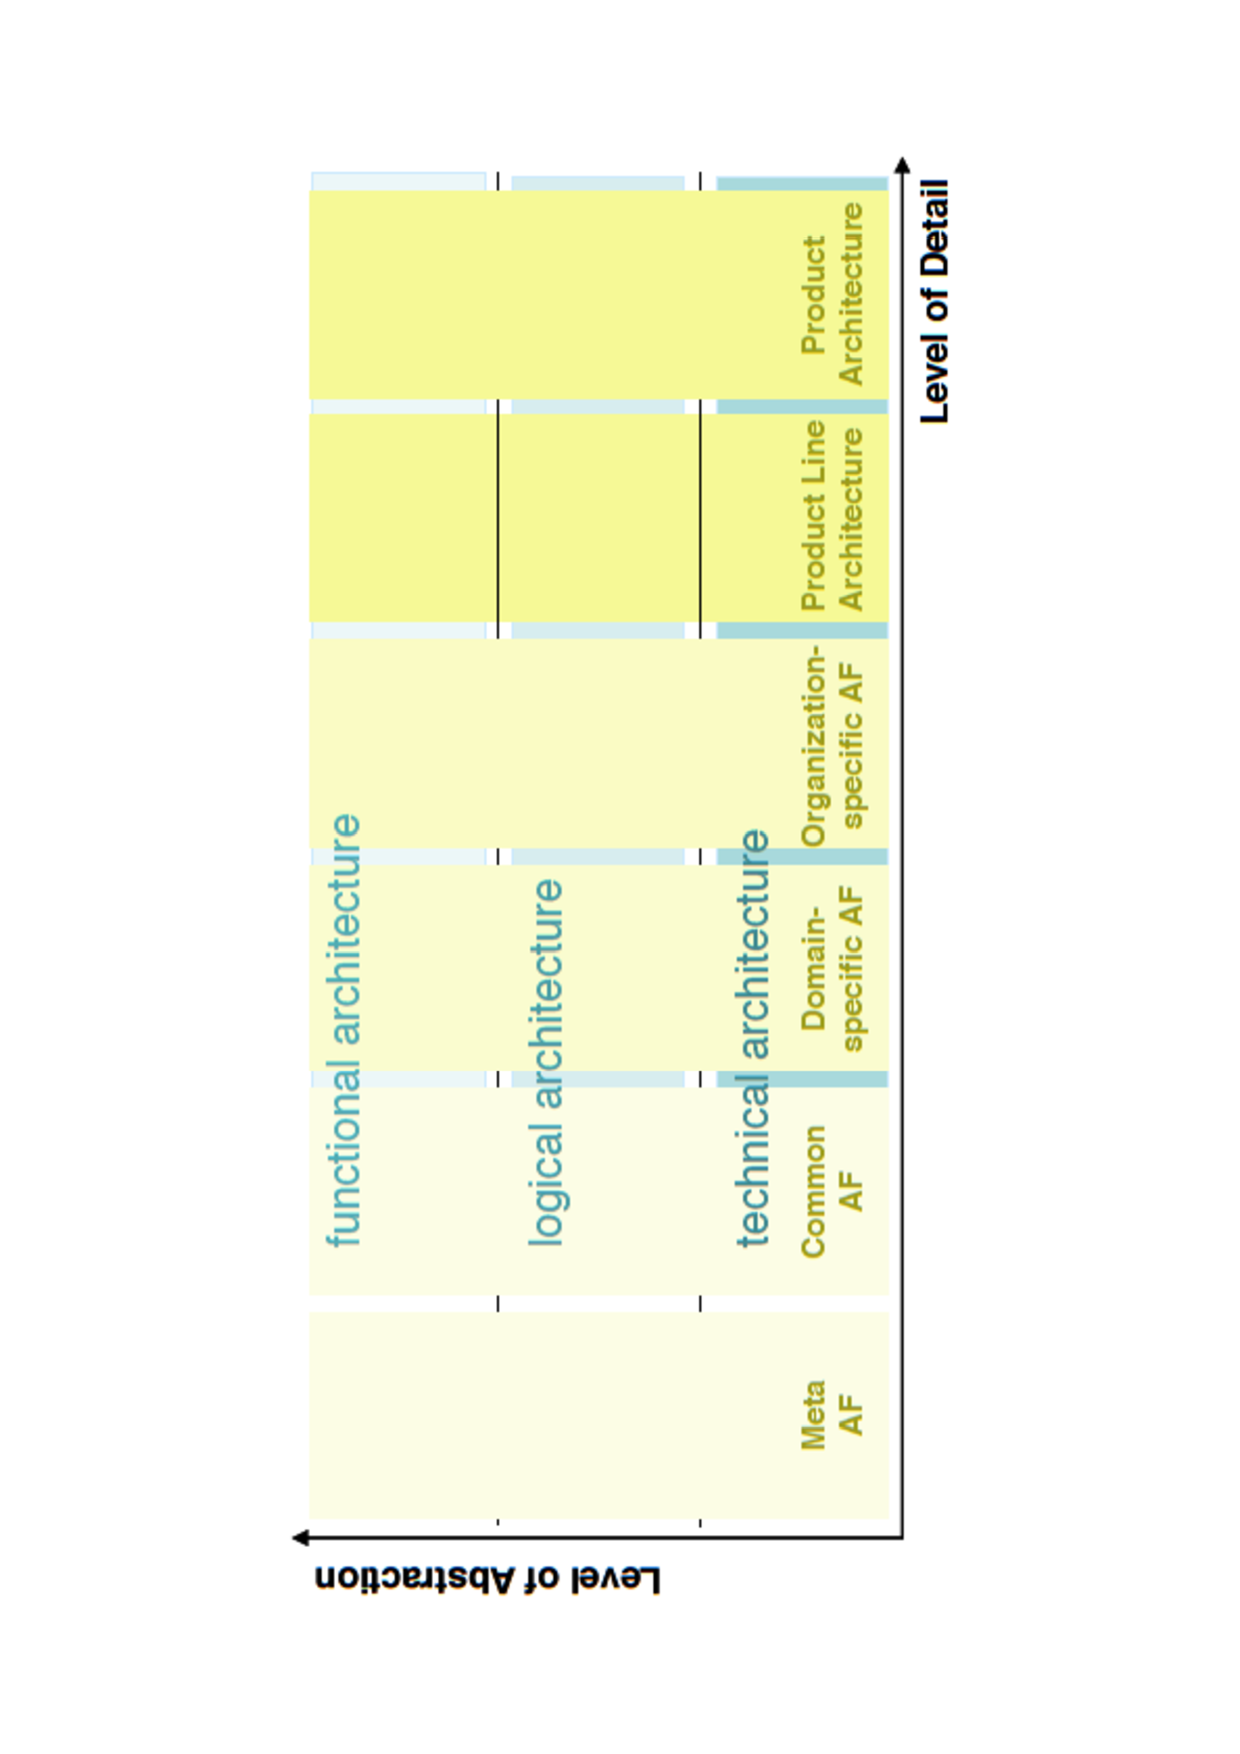
\includegraphics[width=6cm,angle=270]{figures/abstractionDetails.pdf}
%  \caption{Level of Abstraction and Level of Detail - Figure taken from~\cite{TUM-I0915}}
%%  \vspace{-.5cm}
%  \label{fig:abstractionDetails}
%      \end{center}
%\end{figure}


%Focusing on the Domain-specific Architecture Framework for the Automotive Domain, t
The AAF distinguishes between two sets of architecture viewpoints and views: (i) mandatory and general viewpoints and (ii) optional viewpoints. The following viewpoints are presented according to the viewpoint catalog in~\cite{Rozanski2005}.
The mandatory viewpoints and their respective views include: (i)
%
%\begin{itemize} 
%\item 
Functional viewpoint - functional decomposition, functional
architecture;
%\item 
(ii) Logical viewpoint - logical decomposition, logical architecture; this viewpoint is only mentioned in~\cite{Broy} but not detailed in~\cite{TUM-I0915};
%\item 
(iii) Technical viewpoint - physical decomposition, technical architecture;
%\item 
(iv) Information viewpoint - perspective of information or data objects used to
define and manage a vehicle;
%\item 
(v) Driver/vehicle operations viewpoint - vehicle environment;
%\item 
(vi) Value net viewpoint - OEM stakeholders and those of its suppliers and engineering partners. 
%\end{itemize}
The optional viewpoints suggested by the AAF are:
(i) Safety, (ii) Security, (iii) Quality and RAS - Reliability, Availability, Serviceability, (iv) Energy, possibly including performance, (v) Cost, (vi) NVH - noise, vibration, harshness, and (vii) Weight.

\subsection{Architectural Design Framework}

The Architectural Design Framework (ADF)~\cite{AFRenault} is developed by Renault %to support
%the construction of an architecture framework for the automotive industry. The ADF
and 
includes operational, functional, constructional, and requirements viewpoints. Although
the AAF and ADF are related they have some differences. 

\begin{itemize}
\item {\em Operational Viewpoint} - this is the more abstract viewpoint. %The actors, the system scope, the system environment and
%high-level interactions have to be identified; t
The system is observed from a black box and user perspective~\cite{AFRenault}.
\item {\em Functional  Viewpoint} - system functions %are obtained from 
identified in the views associated to the operational viewpoint %and by properly grouping or refining Activities (actions) and allocating them on 
are allocated to SysML Blocks. 
\item {\em Constructional Viewpoint} - this viewpoint %is more detailed and 
describes a further allocation (or grouping) of system functions into physical components.
\item {\em Requirements Viewpoint} - this viewpoint is orthogonal to other viewpoints. Each requirement view has a relationship with views of
other viewpoints. The suggested process is quite waterfall-ish. Stakeholder requirements are built
at the very beginning after the identification of actors and system boundary. These requirements are the starting point for identifying High-
Level Requirements. The Technical Requirement view is typically built 
after the whole set of Operational Views is available.
%\eric{despite being orthogonal, what does this viewpoint do? Description not on same level as other viewpoints.}
\end{itemize}

\subsection{Architecture Framework For Automotive Systems}
The Architecture Framework for Automotive Systems (AFAS) is proposed in~\cite{Yania} through an analysis of AAF, ADF, and of Architecture Description Languages~\cite{ADL_Neno00,whatindustrywants} tailored to automotive domain, like EAST-ADL~\cite{EAST-ADL} %, TADL\footnote{TADL: Timing Augmented Description Language version
%2. \url{http://www.timmo-2-use.org/timmo/index.htm}.}, AADL~\cite{aadl}, 
and AML~\cite{AML}. 
It contains an elaboration and unification of the viewpoints proposed in AAF and ADF and then proposes additional viewpoints, e.g.:

\begin{itemize}
\item {\em Feature viewpoint} - to be used to support the product line engineering. %; it is inspired to~\cite{EAST-ADL}, the only automotive ADL supporting product lines in the architecture description.
\item {\em Implementation viewpoint} - 
it describes the software architecture of the Electrical/Electronic (E/E) system in the vehicle~\cite{EAST-ADL}. %, supported by the system architecture
%and software architecture of AUTOSAR. 
\end{itemize}


